\newpage
\setheaders{Plenary Panel}{\daydateyear}
\section{Plenary Panel}
\index{Matías, Karen}
\index{Somasundaran, Swapna}
\index{Yaneva, Victoria}
\index{Kochmar, Ekaterina}

\begin{center}
{\bfseries\Large Large Language Models (LLMs)\\\vspace{2.0\lineskip}and their Impact on Education} \\
\vspace{1.0em}
{\large\bf Karen Matías, Swapna Somasundaran,\\\vspace{2.0\lineskip}Victoria Yaneva, and Ekaterina Kochmar} \\

\textbf{\daydateyear{}, 11:00--12:30 CST}\\
\textbf{\PlenaryLoc{}}
\end{center}

\noindent
{\bfseries Abstract:}
In this panel discussion, academics will explore the significant impact of Large Language Models (LLMs) on modern-day education. From redefining the assessment of student writing to reshaping the nature of composition, LLMs have sparked a paradigm shift in educational practices. LLMs have also enabled new opportunities in content creation, interactive tutoring, and personalization. The panelists will discuss how LLMs are altering the landscape of education in schools, online education, self-directed learning settings, and high-stakes assessments. This panel will allow attendees to understand the challenges and ethical considerations of integrating LLMs in educational settings. Key questions that the panelist will discuss:
\begin{itemize}
\item How LLMs affect high-stake and student writing assessment
\item How LLMs change writing
\item How LLMs enable new forms of educational applications
\item How LLMs affect educational outcomes
\item How LLMs impact plagiarism detection
\end{itemize}



\vspace{1em}
\begin{center}
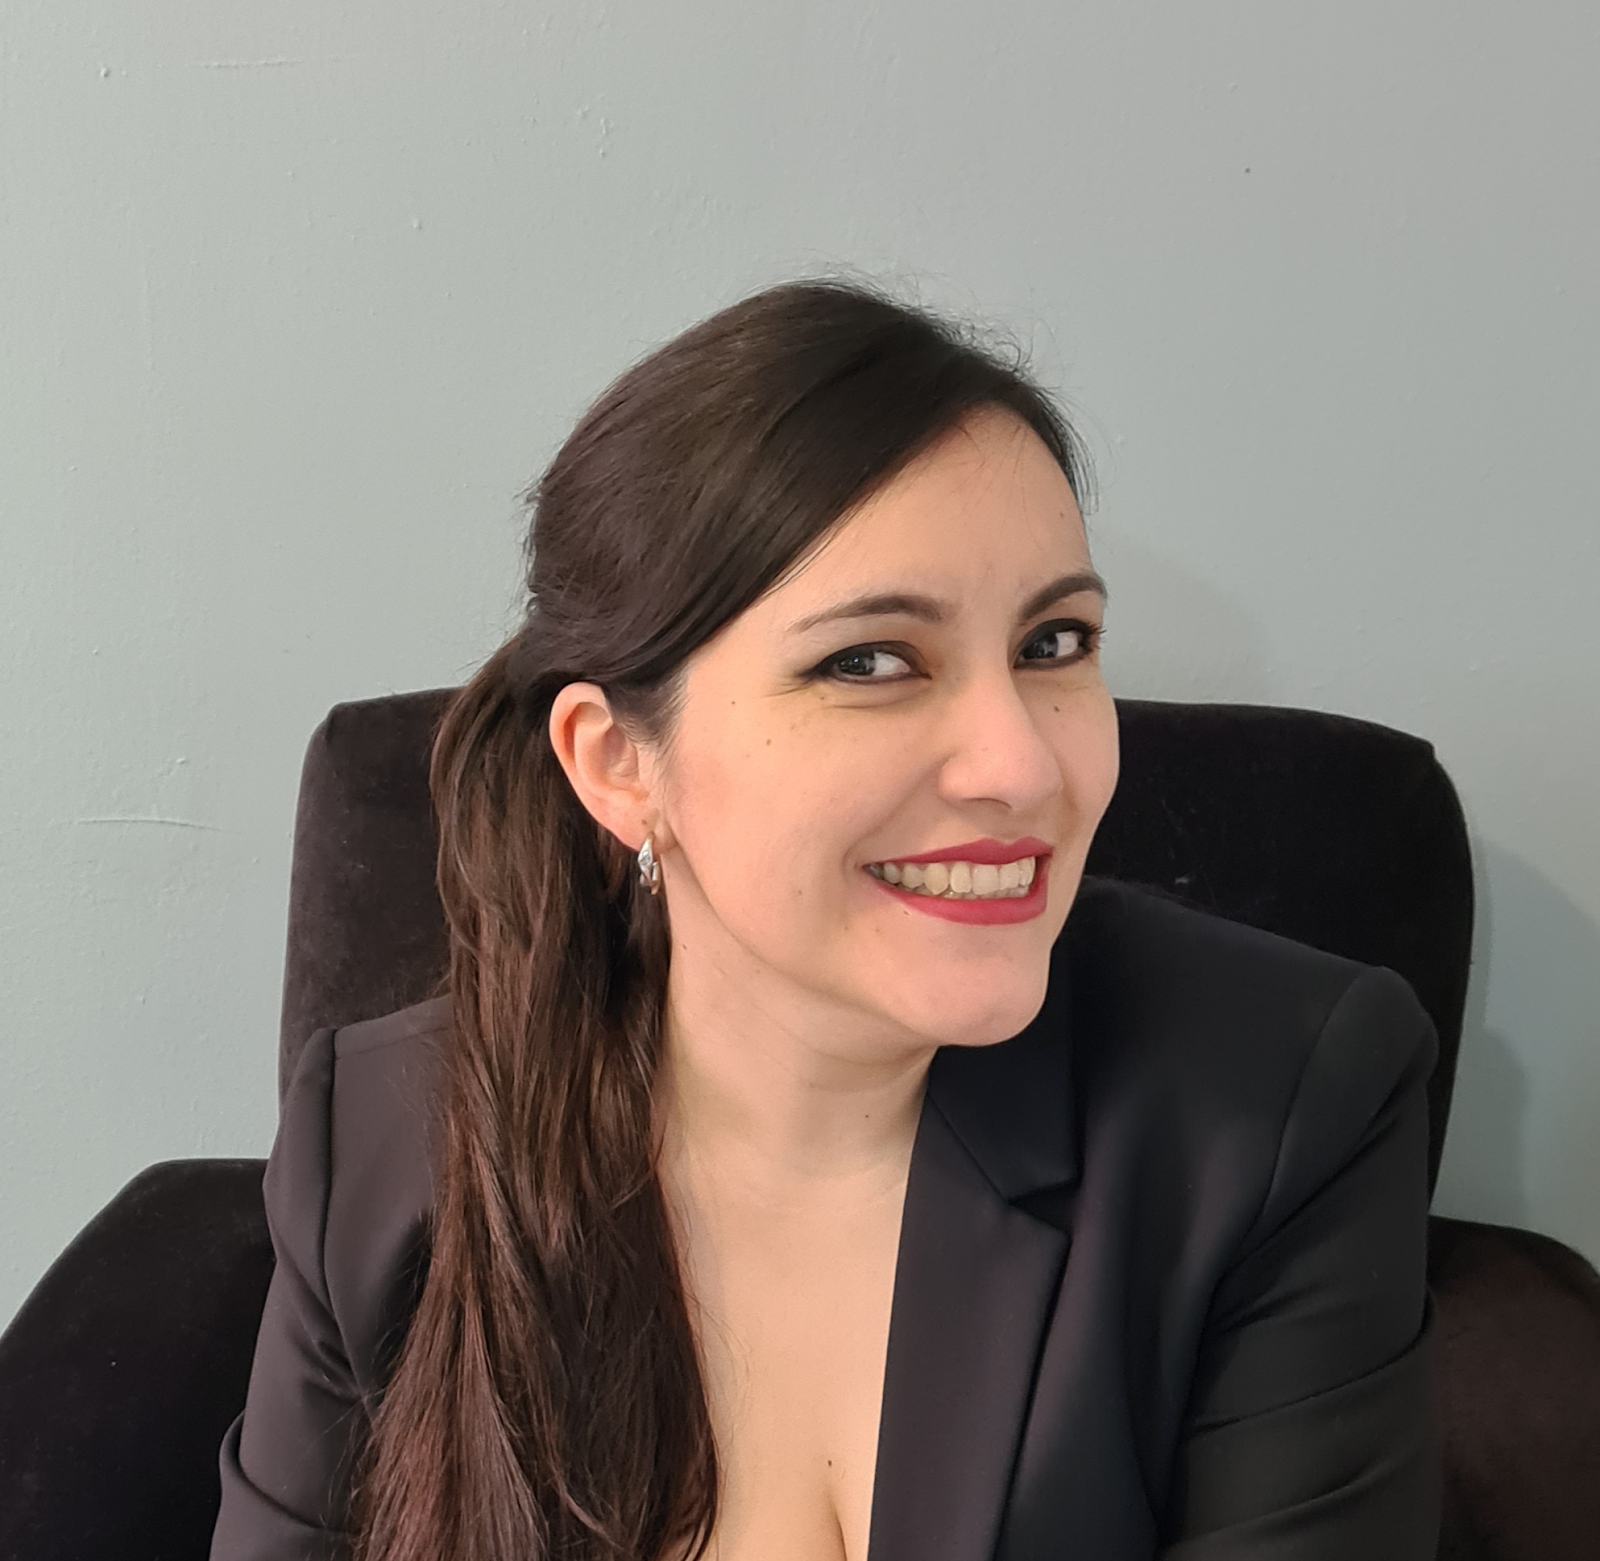
\includegraphics[width=0.4\linewidth]{content/day2/karen.png}
\end{center}
{\bfseries Karen Matías, National Autonomus University of Mexico (UNAM):}
Karen Matias holds a degree in Pedagogy and a specialization in teaching and learning strategies. She completed a specialization in Economic History at the National Autonomous University of Mexico (UNAM) and is currently a candidate for a Master’s degree in Social Philosophy. With over 10 years of experience in educational assessment at both basic and higher education levels, she presently serves as the Head of the Department of Learning Experience Design at UNAM. In this role, she has focused on educational innovation, Artificial Intelligence, and critical thinking. Additionally, she is the Secretary General of the Association of Italian Researchers in Mexico and a member of the Network of Women United for Education. Preferred name (with pronouns): Karen Matias (she/her).

Preferred name (with pronouns): Karen Matias (she/her).


\vspace{1em}
\begin{center}
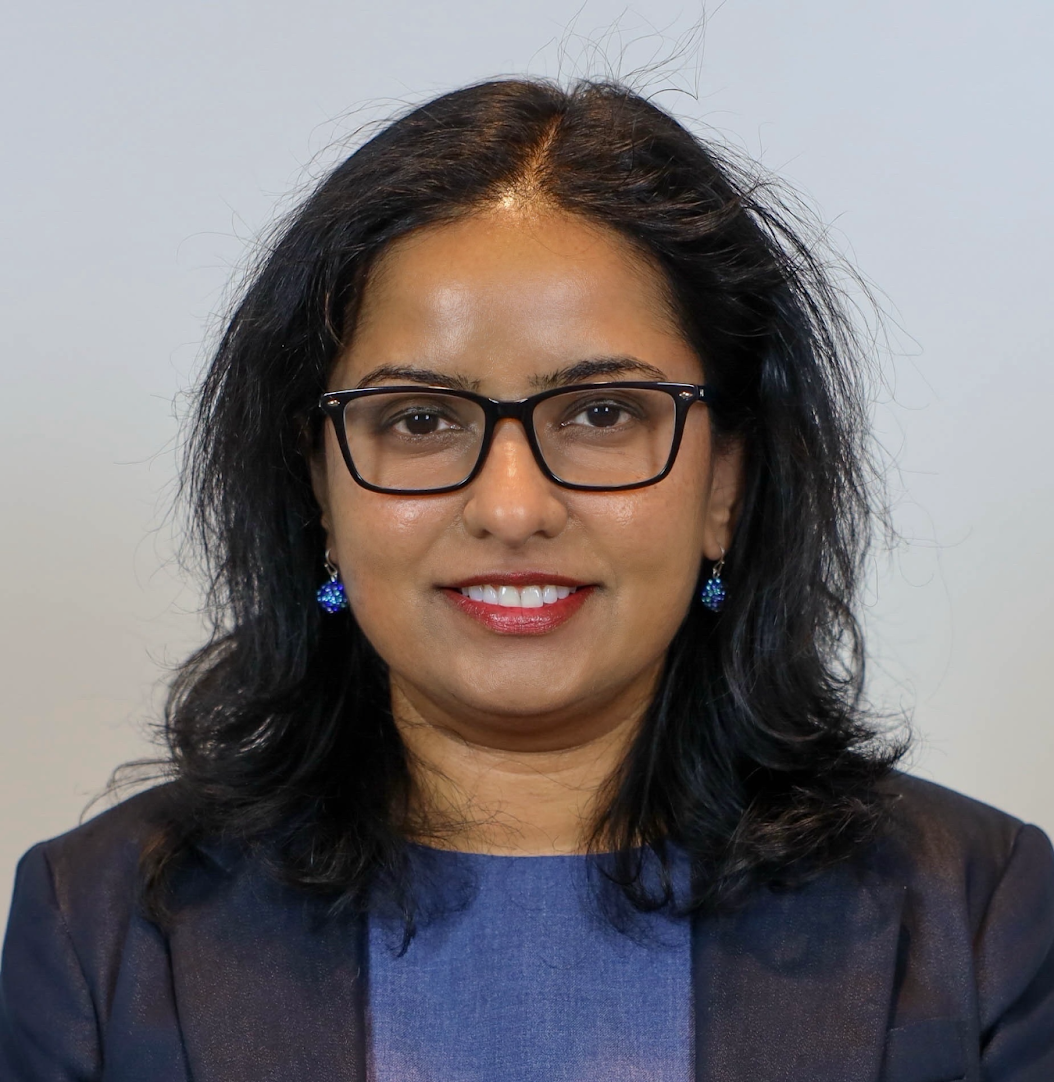
\includegraphics[width=0.4\linewidth]{content/day2/swapna.png}
\end{center}
{\bfseries Swapna Somasundaran - Educational Testing Services (ETS):}
Swapna Somasundaran is the Director of NLP \& Gen AI at Educational Testing Service, where she heads scientists and engineers in product innovations. She also leads the initiative on AI automation of assessments. For over more than a decade, Swapna has worked on NLP problems in the educational domain, from automated scoring using construct-relevant linguistic features to automated creation of assessments using LLMs.

Swapna got her PhD from the University of Pittsburgh. She has a MSE from the Johns Hopkins University and has worked on NLP problems in Healthcare and Energy before joining ETS. Her areas of interest are discourse, sentiment, responsible AI, and equity in education.


\vspace{1em}
\begin{center}
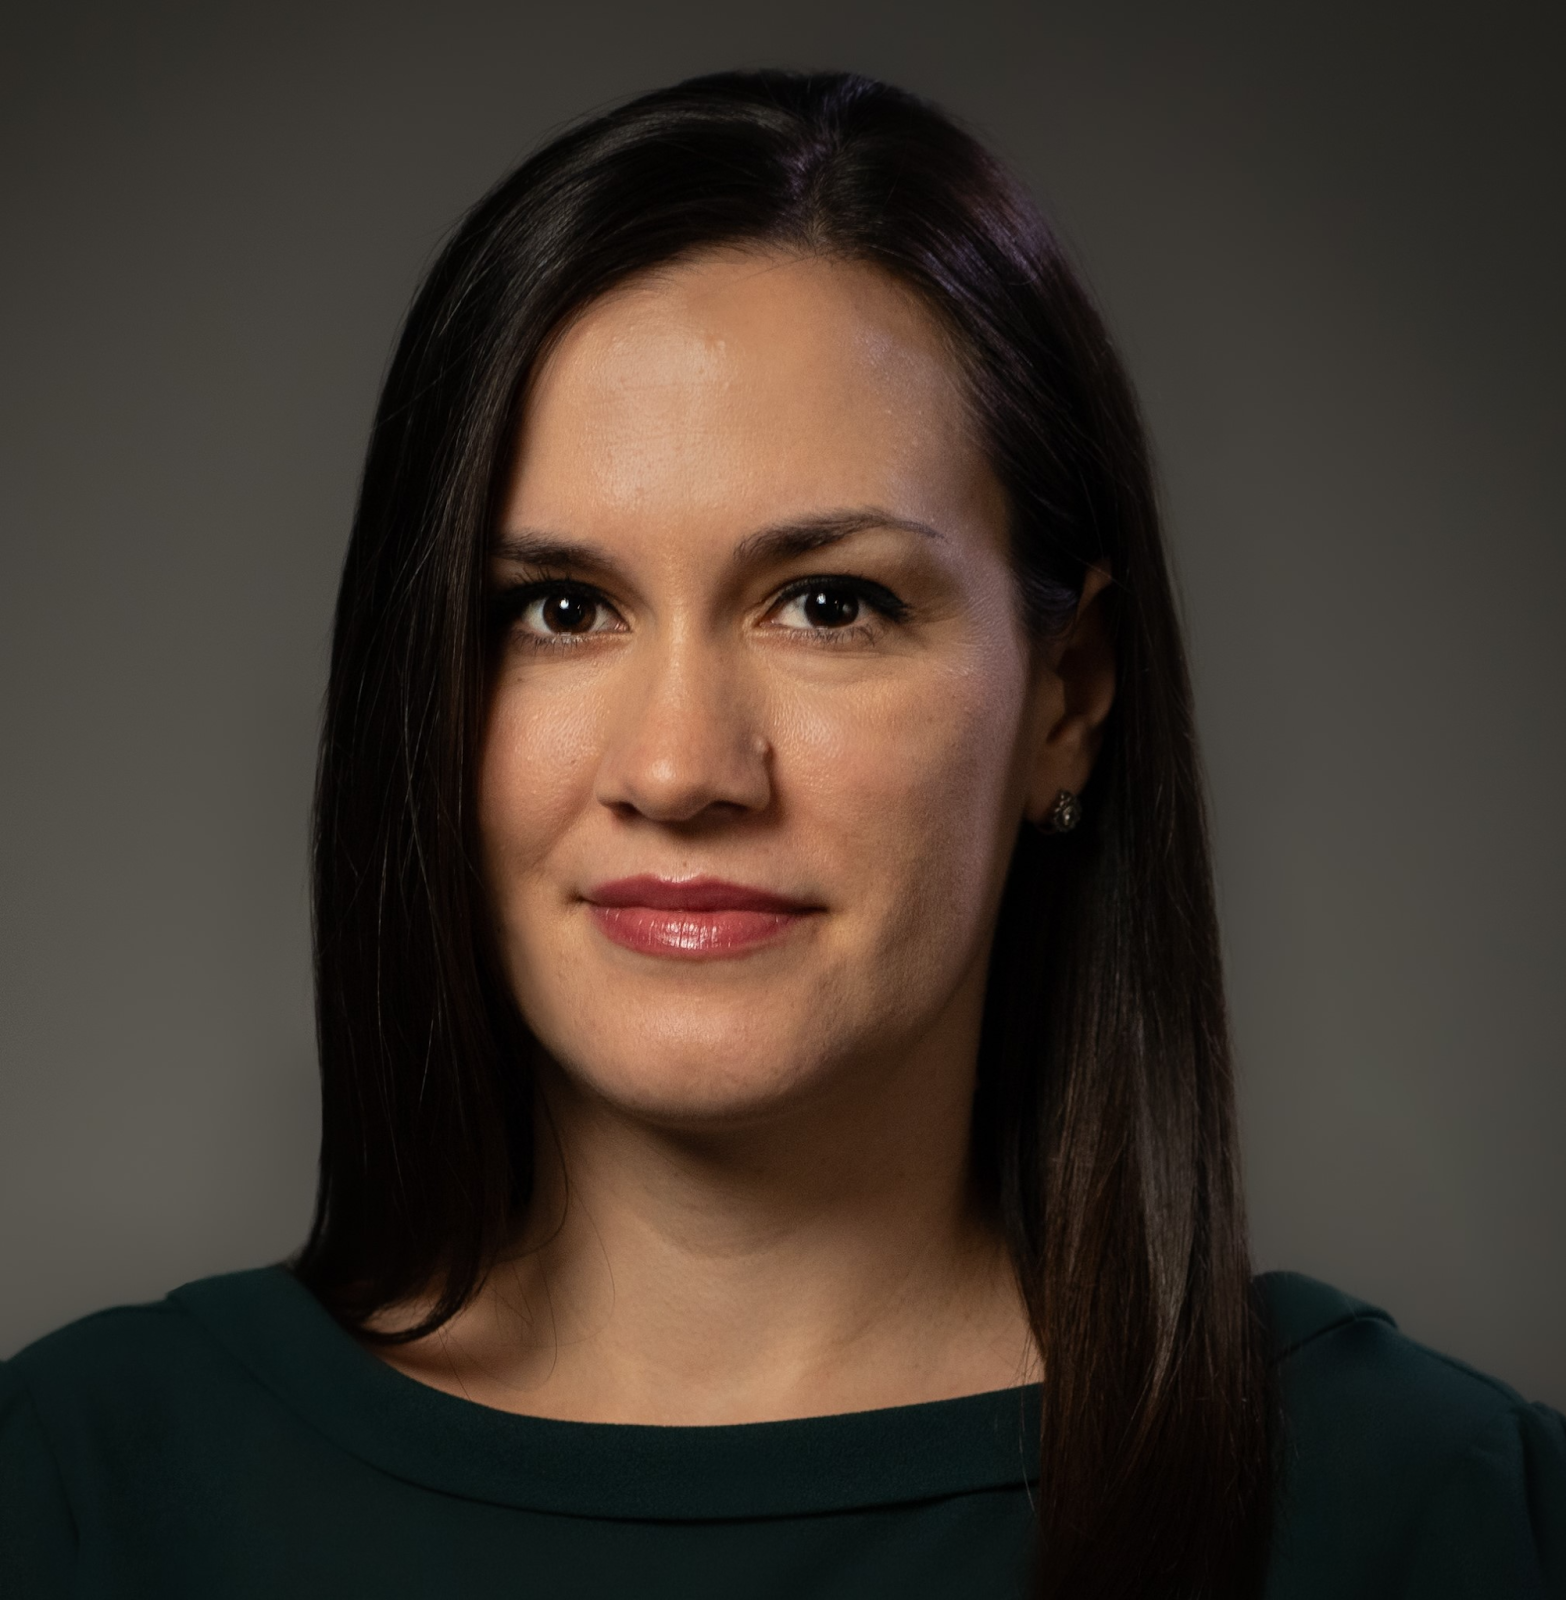
\includegraphics[width=0.4\linewidth]{content/day2/victoria.png}
\end{center}
{\bfseries Victoria Yaneva - National Board of Medical Examiners (NBME):}
Victoria Yaneva is Manager of NLP Research at the National Board of Medical Examiners (NBME). At NBME, Victoria leads a team of NLP scientists conducting research in the intersection between AI/NLP and educational measurement, with an emphasis on developing capabilities for high-stakes clinical exams. Examples include research on LLM-assisted development of exam content, provision of personalized learner feedback, automated prediction of item difficulty, and automated scoring of examinee responses. Another area of interest is the use of behavioral data, such as eye tracking, for investigating the process validity of various types of question formats used in testing. Victoria completed her PhD in NLP at the Research Group in Computational Linguistics at the University of Wolverhampton in 2016. She worked as a postdoctoral researcher in the same research group focusing on accessibility research for people with autism prior to joining NBME in 2018. Victoria has co-authored numerous conference papers and journal articles published in top-tier venues in NLP, educational measurement, medical education, and accessibility. Together with Matthias von Davier, Victoria co-edited the recently released book Advancing Natural Language Processing in Educational Assessment.

Preferred name (with pronouns): Victoria (she/her)


\vspace{1em}
\begin{center}
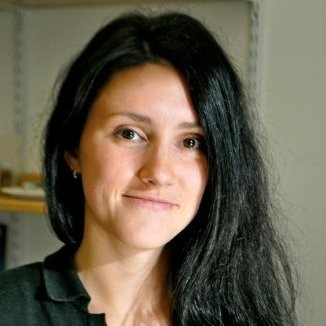
\includegraphics[width=0.4\linewidth]{content/day2/ekaterina.png}
\end{center}
{\bfseries Ekaterina Kochmar - Mohamed bin Zayed University of Artificial Intelligence (MBZUAI):}
Ekaterina Kochmar is an Assistant Professor at the Natural Language Processing Department at MBZUAI, where she conducts research at the intersection of artificial intelligence, natural language processing and intelligent tutoring systems. Previously, she was an Assistant Professor at the University of Bath, where she was part of the AI research group; and prior to that, she was a post-doctoral researcher at the ALTA (Automated Language Teaching and Assessment) Institute, University of Cambridge, focusing on the development of educational applications for second language learners. Her research contributed to the building of Read \& Improve, a readability platform for non-native readers of English. She is the General Chair for the Workshop on Innovative Use of NLP for Building Educational Applications (BEA) and the President of ACL’s SIGEDU. She is also a co-founder and the chief scientific officer of Korbit AI, focusing on building an AI-powered dialogue-based tutoring system capable of providing learners with high-quality, interactive, and personalized education in STEM subjects.

Preferred name (with pronouns): Ekaterina (she/her)


\newpage
